\documentclass[11pt]{charter}

% El títulos de la memoria, se usa en la carátula y se puede usar el cualquier lugar del documento con el comando \ttitle
\titulo{Cargador de Baterías Modular con Monitoreo Remoto} 

% Nombre del posgrado, se usa en la carátula y se puede usar el cualquier lugar del documento con el comando \degreename
\posgrado{Carrera de Especialización en Sistemas Embebidos} 
%\posgrado{Carrera de Especialización en Internet de las Cosas} 
%\posgrado{Carrera de Especialización en Intelegencia Artificial}
%\posgrado{Maestría en Sistemas Embebidos} 
%\posgrado{Maestría en Internet de las cosas}

% Tu nombre, se puede usar el cualquier lugar del documento con el comando \authorname
\autor{Felipe Calcavecchia} 

% El nombre del director y co-director, se puede usar el cualquier lugar del documento con el comando \supname y \cosupname y \pertesupname y \pertecosupname
\director{Alejandro Permingeat}
\pertenenciaDirector{FIUBA} 
% FIXME:NO IMPLEMENTADO EL CODIRECTOR ni su pertenencia
\codirector{} % si queda vacio no se deberíá incluir 
\pertenenciaCoDirector{}

% Nombre del cliente, quien va a aprobar los resultados del proyecto, se puede usar con el comando \clientename y \empclientename
\cliente{Luis A. Rosende}
\empresaCliente{\textit{\textbf{proba}} Baterías}

% Nombre y pertenencia de los jurados, se pueden usar el cualquier lugar del documento con el comando \jurunoname, \jurdosname y \jurtresname y \perteunoname, \pertedosname y \pertetresname.
\juradoUno{Nombre y Apellido (1)}
\pertenenciaJurUno{pertenencia (1)} 
\juradoDos{Nombre y Apellido (2)}
\pertenenciaJurDos{pertenencia (2)}
\juradoTres{Nombre y Apellido (3)}
\pertenenciaJurTres{pertenencia (3)}
 
\fechaINICIO{27 de junio de 2020}		%Fecha de inicio de la cursada de GdP \fechaInicioName
\fechaFINALPlanificacion{22 de Agosto de 2020} 	%Fecha de final de cursada de GdP
\fechaFINALTrabajo{5 de Agosto de 2021}		%Fecha de defensa pública del trabajo final

\usepackage{enumitem}

\begin{document}

\maketitle
\thispagestyle{empty}
\pagebreak


\thispagestyle{empty}
{\setlength{\parskip}{0pt}
\tableofcontents{}
}
\pagebreak


\section{Registros de cambios}
\label{sec:registro}


\begin{table}[ht]
\label{tab:registro}
\centering

\begin{tabularx}{\linewidth}{@{}|c|X|c|@{}}
\hline
\rowcolor[HTML]{C0C0C0} 
Revisión & \multicolumn{1}{c|}{\cellcolor[HTML]{C0C0C0}Detalles de los cambios realizados} & Fecha      \\ \hline

1.0      & Creación del documento          					& 27/06/2020 \\ \hline

1.1      & Se completó Propósito, Alcance, Supuestos, Requerimientos, Entregables y Desglose del trabajo en taréas 								& 10/07/2020 \\ \hline

1.2      & Se Hacen correcciones y se avanza hasta el punto 11 & 23/07/2020 \\ \hline

1.3      & Se avanza hasta el punto 17						 & 7/08/2020 \\ \hline

1.4      & Se agregaron historias de usuarios				 & 8/08/2020 \\ \hline

%		   Con texto partido \newline
%		   En varias líneas \newline
%		   A propósito                                                                     

\end{tabularx}
\end{table}

\pagebreak



\section{Acta de constitución del proyecto}
\label{sec:acta}

\begin{flushright}
Buenos Aires, \fechaInicioName
\end{flushright}

\vspace{2cm}

Por medio de la presente se acuerda con el Ing. \authorname\hspace{1px} que su Trabajo Final de la \degreename\hspace{1px} se titulará ``\ttitle'', consistirá esencialmente en el prototipo preliminar de una fuente utilizada como cargador y una placa de control que garantice la funcionalidad del mismo, y tendrá un presupuesto preliminar estimado de 670 hs de trabajo y {\$845.619}, con fecha de inicio \fechaInicioName\hspace{1px} y fecha de presentación pública \fechaFinalName.

Se adjunta a esta acta la planificación inicial.

\vfill

% Esta parte se construye sola con la información que hayan cargado en el preámbulo del documento y no debe modificarla
\begin{table}[ht]
\centering
\begin{tabular}{ccc}
\begin{tabular}[c]{@{}c@{}}Ariel Lutenberg \\ Director posgrado FIUBA\end{tabular} &  & \begin{tabular}[c]{@{}c@{}}\clientename \\ \empclientename \end{tabular} \vspace{2.5cm} \\ 
\multicolumn{3}{c}{\begin{tabular}[c]{@{}c@{}} \supname \\ Director del Trabajo Final\end{tabular}} \vspace{2.5cm} \\
\begin{tabular}[c]{@{}c@{}}\jurunoname \\ Jurado del Trabajo Final\end{tabular}     &  & \begin{tabular}[c]{@{}c@{}}\jurdosname\\ Jurado del Trabajo Final\end{tabular}  \vspace{2.5cm}  \\
\multicolumn{3}{c}{\begin{tabular}[c]{@{}c@{}} \jurtresname\\ Jurado del Trabajo Final\end{tabular}} \vspace{.5cm}                                                                     
\end{tabular}
\end{table}




\section{Descripción técnica-conceptual del proyecto a realizar}
\label{sec:descripcion}

Hoy en día las baterías de uso industrial constituyen una parte fundamental en sistemas de respaldo de alimentación, vehículos de tracción eléctrica y otros múltiples usos. Su elevado costo respecto de los  dispositivos que alimentan, hacen que un buen uso y mantenimiento sea una cuestión a tener en cuenta a la hora de considerar su vida útil.
\\[3pt]
Todo esto lleva a la necesidad de desarrollar un cargador que asegure una carga adecuada (en tensión y corriente), de acuerdo al tipo de batería, a su estado de carga y a las condiciones ambientales que la rodean.
\\[3pt]
Si tenemos en cuenta que el mercado local ofrece algunos cargadores nacionales, la mayoría se basan en tecnologías antiguas. Por el lado de los importados, tecnológicamente mas avanzados, necesitan certificaciones aduaneras que elevan su precio.
\\[3pt]
Si bien la empresa produce cargadores, estos son un complemento en la comercialización de baterías para automóviles. Con este proyecto se pretende aumentar la presencia de la compañía en el segmento del mercado que corresponde a las baterías industriales expandiendo su modelo de negocio a otras áreas menos explotadas.\\ 
En la Figura \ref{fig:modeloCanvas} se puede observar el modelo Canvas de negocio.

\begin{figure}[h]
\centering 
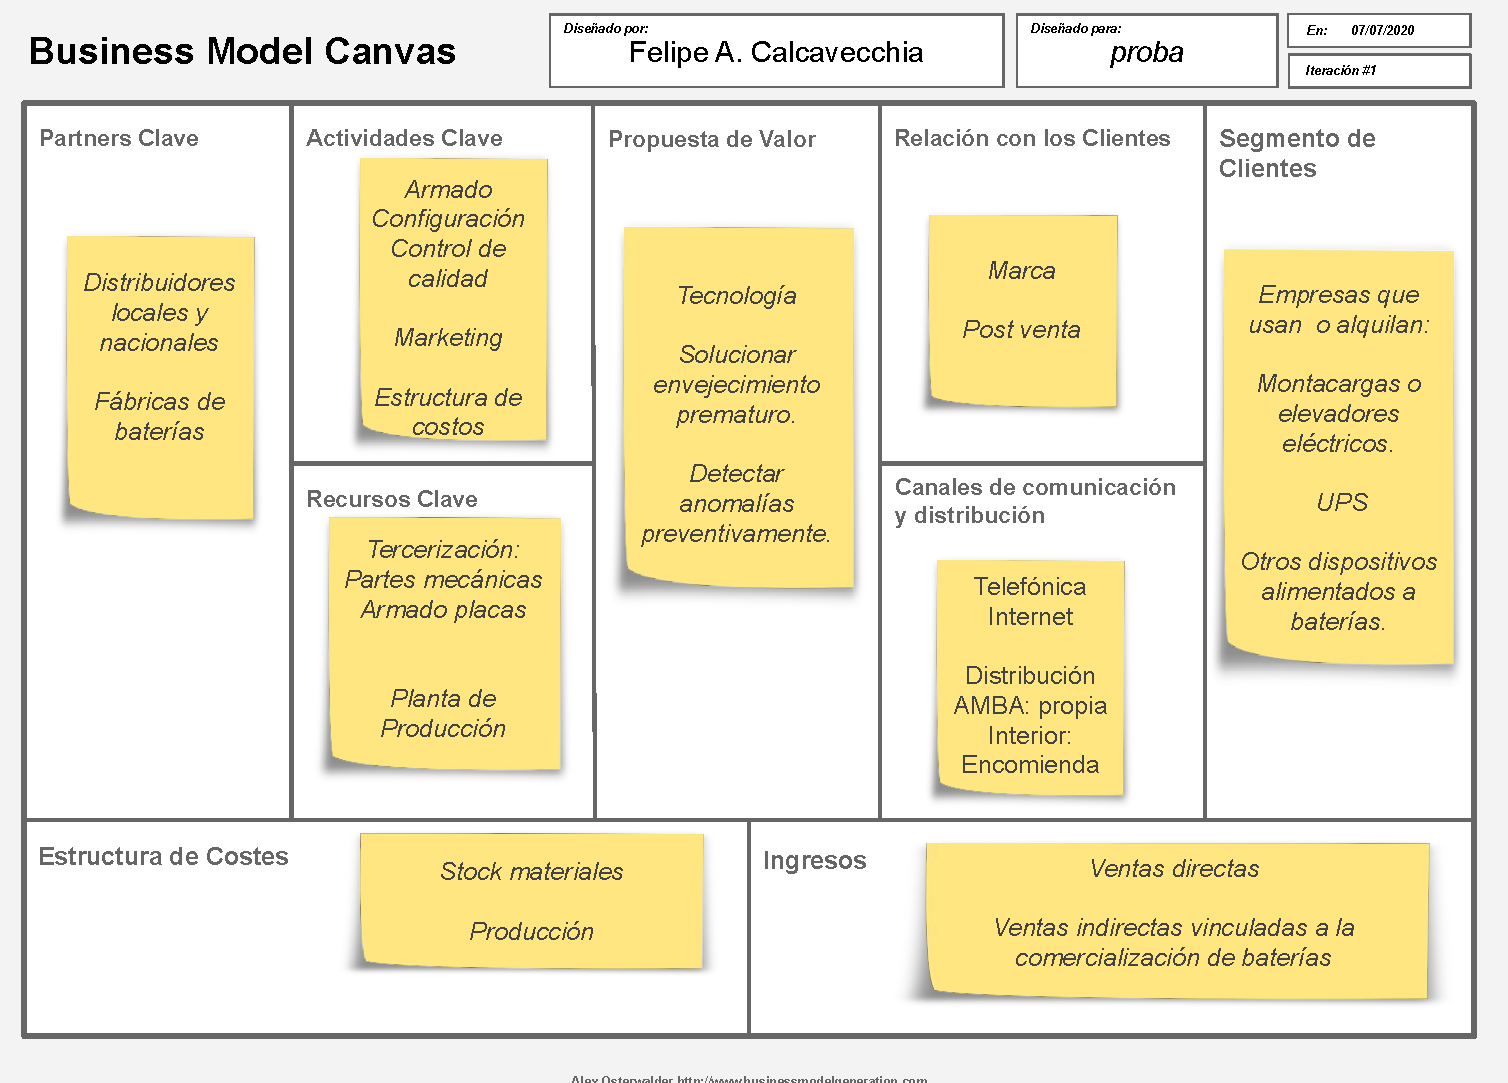
\includegraphics[width=.9\textwidth]{./Figuras/Canvas1.pdf}
\caption{Modelo Canvas de negocio}
\label{fig:modeloCanvas}
\end{figure}

El presente proyecto se destaca en tres aspectos que le agregan valor, dos enfocados en el consumidor final y uno en el cliente.
\\[3pt]
En lo pertinente al consumidor final, y desde el punto de vista del hardware, se reemplazan los voluminosos y pesados transformadores por fuentes conmutadas de alta frecuencia, mas eficaces, pequeñas y livianas.\\
Desde el lado del firmware de control, este, permite adaptarse a cada tipo de banco de baterías en forma particular. Además como aspecto innovador, se incorpora un monitoreo de cada una de las cargas que realiza y con esa información genera un log que permite hacer un análisis periódico del estado de la batería y activar alarmas tempranas en caso de detectar alguna anomalía.
\\[3pt]
Por el lado del cliente, se beneficia al disminuir stock inmovilizado, teniendo un solo modelo de cargador modularizado y configurable, en vez de varios cargadores, uno por cada tipo de batería, simplificando su producción y ahorrando costos.

En la Figura \ref{fig:diagBloques} se muestra el diagrama en bloques del proyecto a realizar. Se observa que el cargador posee una disposición modular en la que admite 1, 2 ó 3 fuentes. Cada una puede aportar hasta 40 Amperes. Esto posiblita configurar el cargador para adaptarse a los requerimientos de los distintos tipos de baterías, abarcando las tensiones standards más utilizadas (12V, 24V, 36V y 48V) y corrientes de carga que pueden ir desde 1A hasta 120A.\\[3pt]
La placa que controla al cargador contiene un microprocesador capaz de suministrar tres señales PWM independientes  que manejan las tensiones de salidas de las tres fuentes, cinco canales ADC para leer sensores, un puerto con entradas/salidas digitales para el display, teclado, relés de alarma y otros accesorios como indicadores luminosos, ventiladores, etc, y por último una comunicacion serie para los módulos de WIFI y el reloj de tiempo real.\\[3pt]
El firmware controla, en forma secuencial, cuatro etapas de carga:

%\vspace{5px}

\begin{figure}[htpb]
\centering 
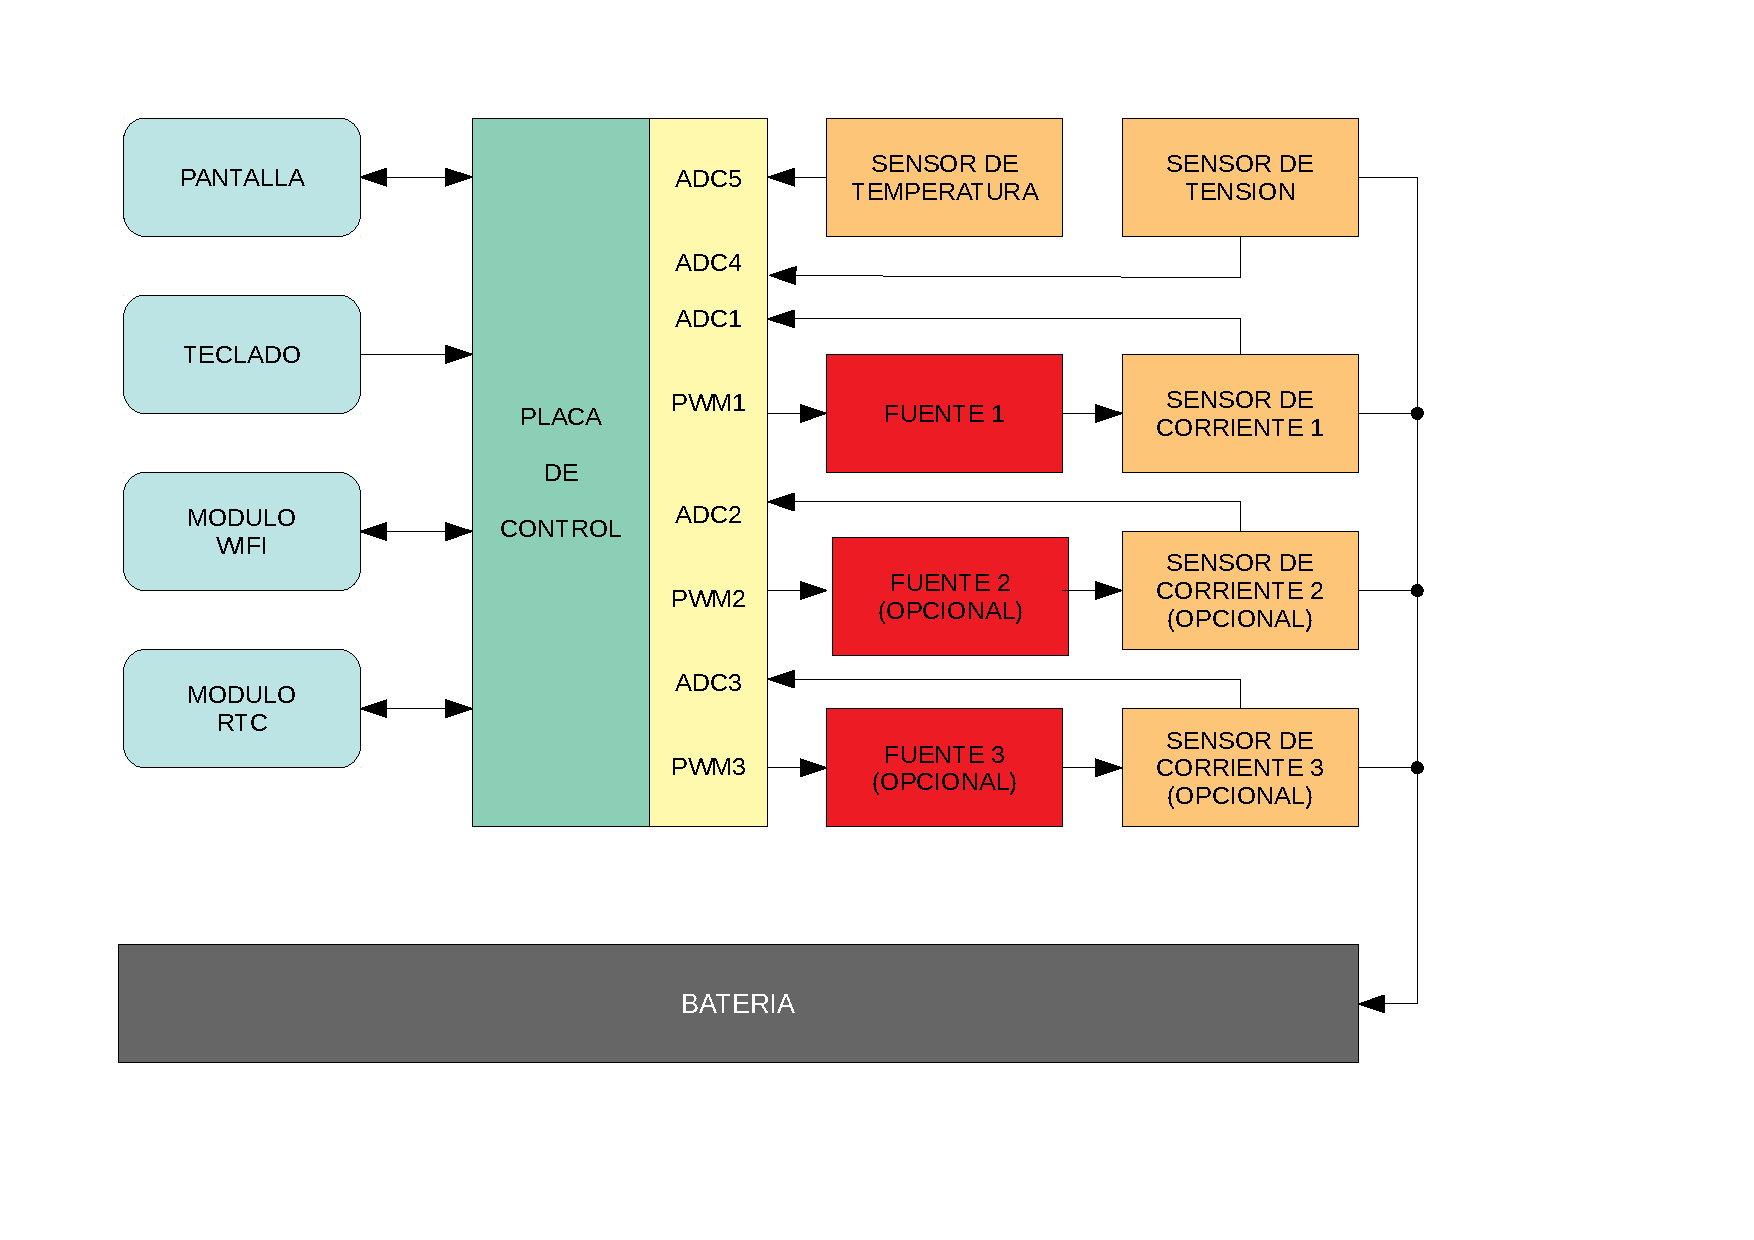
\includegraphics[width=.8\textwidth]{./Figuras/Plan_Figura1.pdf}
\caption{Diagrama en bloques del sistema}
\label{fig:diagBloques}
\end{figure}

%\vspace{5px}

\begin{enumerate}
\item CARGA A FONDO: Suministra aproximadamente el 80\% de la carga total, se realiza a corriente constante y se registra el tiempo de duración.
\item CARGA POR ABSORCIÓN: Le entrega el 20\% restante de carga y se realiza a tensión constante. Dura aproximadamente el mismo tiempo que la carga a Fondo.
\item CARGA A FLOTE: Cuando finaliza la carga, se fija una tensión y corriente máxima de forma que la batería pueda quedar conectada al cargador indefinidamente sin provocar sobrecargas.
\item ECUALIZACIÓN: Cada un número determinado de cargas, se realiza este paso para equilibrar los elementos que conforman la batería. Se hace forzando una sobrecarga durante un tiempo controlado relativamente corto.
\end{enumerate}

Las corrientes de las fuentes son medidas y comparadas con las de referencia, generando una señal de error que se usa para actuar sobre los PWM’s formando un sistema de lazo cerrado que se controla por un algoritmo PID.
Al finalizar la carga, se genera un registro identificando parámetros como, tensión, corriente, fecha y hora de inicio y finalización, Ampere-Hora suministrado, temperatura y cantidad de cargas realizadas. Estos datos sirven para llevar una “historia clínica” de la batería y verificar si existe alguna anomalía para activar las correspondientes alarmas.

%\clearpage
%\newpage

\section{Identificación y análisis de los interesados}
\label{sec:interesados}



\begin{table}[ht]
%\caption{Identificación de los interesados}
%\label{tab:interesados}
\begin{tabularx}{\linewidth}{@{}|l|X|X|l|@{}}
\hline
\rowcolor[HTML]{C0C0C0} 
Rol           & Nombre y Apellido & Organización 	   & Puesto 	\\ \hline
Auspiciante   &                   &              	   &        	\\ %\hline
Cliente       & \clientename      &\empclientename	   & Dto. Ventas       	\\ %\hline
Impulsor      &                   &              	   &        	\\ \hline
			  &					  &					   &			\\
Responsable   & \authorname       & \textbf{\textit{proba}} Instrumentos       	   & Ing. Desarrollo	\\ 
			  &					  &					   &			\\ \hline
			  &					  &					   &			\\			  
Equipo		  & Luca Calcavecchia & UTN-FRH       	   & Alumno    	\\ 
			  &					  &					   &			\\ \hline
			  &					  &					   &			\\			  
Orientador    & \supname	      & \pertesupname 	   & Director	Trabajo final \\       			  &					  &					   &			\\ \hline
%Equipo        & miembro1 \newline 
%				miembro2          &              	   &        	\\ \hline
%Opositores    &                   &              	   &        	\\ \hline
			  &					  &					   &			\\
Usuario final & Empresas		  & \hspace{2cm}-	   & \hspace{1.8cm}-			\\ 
			  &					  &					   &			\\ \hline
\end{tabularx}
\end{table}

\begin{itemize}
\item[•] El Auspiciante, Cliente e Impulsor es el titular de \textbf{\textit{proba}} Baterías y socio con el Responsable del proyecto en \textbf{\textit{proba}} Instrumentos.
\item[•] El Equipo se encarga del diseño del gabinete y la documentación correspondiente.
\end{itemize}


\section{1. Propósito del proyecto}
\label{sec:proposito}

\begin{consigna}{black}
El propósito de este proyecto es diseñar e implementar un prototipo funcional de un cargador de baterías modular, aplicando los conocimiento que se van adquiriendo en el curso. A su vez que esos conocimientos sirvan para ser incorporados como metodología de trabajo a futuros productos realizados en la empresa.
\end{consigna}

\section{2. Alcance del proyecto}
\label{sec:alcance}

Este proyecto incluirá el diseño y construcción de un prototipo funcional de un cargador de baterías que conste de un sistema embebido formado por una placa, que interactúe con sus periféricos y controle las fuentes de carga. También  se incluirá toda la documentación y archivos necesarios para su producción, así como también su manual de uso e instalación.

No queda incluido en el presente proyecto, el diseño y construcción de las fuentes, el diseño del gabinete y partes mecánicas. Tampoco incluye la implementación de una aplicación de software para la lectura remota del reporte de cargas. Solo se enviarán los datos crudos del log.


\section{3. Supuestos del proyecto}
\label{sec:supuestos}

Para el desarrollo del presente proyecto se supone que: 

\begin{enumerate}
\item Se dispondrá de la información de marketing de los posibles usuarios para analizar las funcionalidades del proyecto.
\item Se contará con los suficientes recursos económicos para la compra de todo el material necesario.
\item Se supone que los componentes a utilizar se consiguen localmente o que se dispone de todos los requisitos necesarios para su importación en caso de ser necesario.
\item Se supone que las fuentes a utilizar tienen el correspondiente certificado de seguridad eléctrica.
\item Se supone que los tiempos de importación están dentro de lo planificado.
\item Se supone que los tiempos de fabricación están dentro de lo planificado.
\item Se supone que se tendrá acceso a las instalaciones y elementos necesarios para realizar las pruebas de campo.
\item Debido a que las pruebas de campo son de larga duración, se dispondrá del tiempo necesario para usar las instalaciones sin restricciones.

\end{enumerate}


\section{4. Requerimientos}
\label{sec:requerimientos}

Los requerimientos del presente proyecto se establecieron luego de acordar con el cliente y muchos a sugerencia de posibles usuarios finales. Los mismos se describen a continuación en orden prioritario.


\begin{enumerate}
	\item \textbf{Requerimientos generales del proyecto}
	\begin{enumerate}[label*=\arabic*.]
		\item Fecha de entrega del proyecto terminado: 5 de Julio de 2021
		\item El responsable asegura al cliente el know-how del proyecto.
		\item Podrá alimentarse con línea de red monofásica o trifásica.
		\item Deberá contemplar protecciones de alimentación a través de llaves térmicas. 
	\end{enumerate}

	\item \textbf{Requerimientos funcionales}
	\begin{enumerate}[label*=\arabic*.]
		\item \textbf{Requerimientos de Hardware}
			\begin{enumerate}[label*=\arabic*.]
				\item El dispositivo debe contemplar un diseño modular.
				\item El diseño modular debe permitir su reconfiguración.
				\item Debe tener un teclado accesible para su configuración y manejo.
				\item Debe poseer un display que permita visualizar la configuración y parámetros mensurables.
				\item Debe poseer indicadores luminosos bien visibles.					
				\item Cada fuente debe tener su propio sensor de corriente.
				\item El sensor de tensión es común a todas las fuentes.
				\item Se agrega un botón de parada de emergencia.			
			\end{enumerate}
		\item \textbf{Requerimientos de Firmware}
			\begin{enumerate}[label*=\arabic*.]
				\item Debe permitir configurar la tensión y corriente máxima de carga.
				\item Debe permitir configurar los tiempos máximos para cada etapa de carga.
				\item Debe guardar al menos dos configuraciones.
				\item Tendrá que medir tensión, corriente y temperatura.
				\item Tendrá que garantizar cuatro etapas de carga:
					\begin{enumerate}[label*=\arabic*.]
						\item Carga a Fondo.
						\item Carga por Absorción.
						\item Carga a Flote.
						\item Ecualización.
					\end{enumerate}
				\item Tendrá un algoritmo que atienda al botón de parada de emergencia.
				\item El control de carga se realizará por un algoritmo PID
				\item Se registrará la fecha y hora de inicio y finalización de cada carga a través de un RTC.
				\item Debe guardar las últimas mil cargas realizadas.
				\item Con los datos recavados se podrá determinar anomalías y generar alarmas. 
				\item El registro de datos almacenados debe estar disponible para ser consultado remotamente.
			\end{enumerate}					
	\end{enumerate}
	\item \textbf{Requerimientos no funcionales}
	\begin{enumerate}[label*=\arabic*.]
		\item Se deberá generar documentación:
			\begin{enumerate}[label*=\arabic*.]
				\item Esquemáticos eléctricos.
				\item Manual de instalación.
				\item Manual de uso.
			\end{enumerate}
		\item Se contará con la correspondiente certificación eléctrica otorgada por un laboratorio habilitado para la importación de las fuentes de carga.
		\item El grado de protección del sistema debe ser como mínimo IP50.
		\item Se debe garantizar un servicio de post venta por al menos 5 años.
	\end{enumerate}
\end{enumerate}

\newpage

\section{Historias de usuarios (\textit{Product backlog})}
\label{sec:backlog}

Se dará una visión de las funcionalidades esperada por distintos usuarios del producto.
A cada historia se le asocia un grado de ponderación de acuerdo a un criterio definido y una prioridad respecto al resto.

Para la ponderación se usarán 3 niveles: 1, 3 y 7. \\
Mientras que para la prioridad se usará de 1 a 5, siendo 1 la prioridad mas baja.
 \\
 
\begin{table}[H]
\resizebox{\textwidth}{!}{%
\begin{tabular}{|l|c|l|c|l|l|}
\hline
\multicolumn{3}{|l|}{\cellcolor[HTML]{C0C0C0}\textbf{Historia de uso 1:}} & \multicolumn{3}{c|}{\cellcolor[HTML]{C0C0C0}\textbf{\begin{tabular}[c]{@{}c@{}}Como operario desearía una conexión rápida entre el cargador\\y la batería\end{tabular}}} \\ \hline
\begin{tabular}[c]{@{}l@{}}Criterio\\ adoptado\end{tabular}    & \multicolumn{5}{l|}{\begin{tabular}[c]{@{}l@{}}Complejidad: baja, si se utilizan conectores rápidos\\ entre el cargador y la batería\end{tabular}}                  \\ \hline
Ponderación                                                    & 1   & \multicolumn{4}{l|}{Es de fácil aplicación}                                                                                                                   \\ \hline
Prioridad                                                      & 2   & \multicolumn{4}{l|}{Hace a la prestación del producto pero no es determinante}                                                                                                        \\ \hline
\end{tabular}%
}
\end{table}

\vspace{3mm}

\begin{table}[H]
\resizebox{\textwidth}{!}{%
\begin{tabular}{|l|c|l|c|l|l|}
\hline
\multicolumn{3}{|l|}{\cellcolor[HTML]{C0C0C0}\textbf{Historia de uso 2:}} & \multicolumn{3}{c|}{\cellcolor[HTML]{C0C0C0}\textbf{\begin{tabular}[c]{@{}c@{}}Como personal de mantenimiento desearía que el equipo sea más\\ liviano y pequeño que el tradicional cargador a transformador\end{tabular}}} \\ \hline
\begin{tabular}[c]{@{}l@{}}Criterio\\ adoptado\end{tabular}    & \multicolumn{5}{l|}{\begin{tabular}[c]{@{}l@{}}Incertidumbre: media, por tratarse de un criterio subjetivo \end{tabular}}                  \\ \hline
Ponderación                                                    & 3   & \multicolumn{4}{l|}{Por ser un valor subjetivo es difícil ponderar}                                                                                                                   \\ \hline
Prioridad                                                      & 1   & \multicolumn{4}{l|}{De por si es inherente al diseño ya que se usan fuentes conmutadas}                                                                                                        \\ \hline
\end{tabular}%
}
\end{table}

\vspace{3mm}

\begin{table}[H]
\resizebox{\textwidth}{!}{%
\begin{tabular}{|l|c|l|c|l|l|}
\hline
\multicolumn{3}{|l|}{\cellcolor[HTML]{C0C0C0}\textbf{Historia de uso 3:}} & \multicolumn{3}{c|}{\cellcolor[HTML]{C0C0C0}\textbf{\begin{tabular}[c]{@{}c@{}}Como administrador desearía hacer un seguimiento del historial de\\cargas de la batería\end{tabular}}} \\ \hline
\begin{tabular}[c]{@{}l@{}}Criterio\\ adoptado\end{tabular}    & \multicolumn{5}{l|}{\begin{tabular}[c]{@{}l@{}}Conocimiento: alto, es un criterio innovador del proyecto \end{tabular}}                  \\ \hline
Ponderación                                                    & 7   & \multicolumn{4}{l|}{Es un factor preponderante en la funcionalidad del sistema }                                                                                                                   \\ \hline
Prioridad                                                      & 5   & \multicolumn{4}{l|}{Es lo que diferenciará este producto del resto de la competencia}                                                                                                        \\ \hline
\end{tabular}%
}
\end{table}

\vspace{3mm}

\begin{table}[H]
\resizebox{\textwidth}{!}{%
\begin{tabular}{|l|c|l|c|l|l|}
\hline
\multicolumn{3}{|l|}{\cellcolor[HTML]{C0C0C0}\textbf{Historia de uso 4:}} & \multicolumn{3}{c|}{\cellcolor[HTML]{C0C0C0}\textbf{\begin{tabular}[c]{@{}c@{}}Como ingeniero de desarrollo desearía tener acceso al historial de\\ carga para mejorar los diagnósticos de fallas\end{tabular}}} \\ \hline
\begin{tabular}[c]{@{}l@{}}Criterio\\ adoptado\end{tabular}    & \multicolumn{5}{l|}{\begin{tabular}[c]{@{}l@{}}Volumen: es un trabajo para subdividirlo en varias etapas\\utilizando estadística para llevarlo a cabo \end{tabular}}                  \\ \hline
Ponderación                                                    & 3   & \multicolumn{4}{l|}{Hace a la sostenibilidad del producto }                                                                                                                   \\ \hline
Prioridad                                                      & 3   & \multicolumn{4}{l|}{De la investigación pueden surgir nuevas funcionalidades y/o productos}                                                                                                        \\ \hline
\end{tabular}%
}
\end{table}

\vspace{3mm}

\begin{table}[H]
\resizebox{\textwidth}{!}{%
\begin{tabular}{|l|c|l|c|l|l|}
\hline
\multicolumn{3}{|l|}{\cellcolor[HTML]{C0C0C0}\textbf{Historia de uso 5:}} & \multicolumn{3}{c|}{\cellcolor[HTML]{C0C0C0}\textbf{\begin{tabular}[c]{@{}c@{}}Como técnico desearía un cargador configurable que se adapte a\\ cualquier tipo de batería \end{tabular}}} \\ \hline
\begin{tabular}[c]{@{}l@{}}Criterio\\ adoptado\end{tabular}    & \multicolumn{5}{l|}{\begin{tabular}[c]{@{}l@{}}Complejidad: media, se puede alcanzar agregando código adicional \end{tabular}}                  \\ \hline
Ponderación                                                    & 7   & \multicolumn{4}{l|}{Hace del cargador un producto flexible y adaptable.}                                                                                                                   \\ \hline
Prioridad                                                      & 4   & \multicolumn{4}{l|}{Es otro de los factores que le da valor agregado al producto}                                                                                                        \\ \hline
\end{tabular}%
}
\end{table}


\section{5. Entregables principales del proyecto}
\label{sec:entregables}


\begin{itemize}
\item Plan de trabajo
\item Memoria del proyecto
\item Prototipo funcional
\item Diagrama esquemático
\item Manual de instalación
\item Manual de uso
\item Código fuente
 
\end{itemize}

\section{6. Desglose del trabajo en tareas}
\label{sec:wbs}

\begin{enumerate}
	\item \textbf{Planificación del proyecto (30hs)}
	\begin{enumerate}[label*=\arabic*.]
		\item Definición de requerimientos con el cliente (15hs)
		\item Confección del plan de trabajo (15hs)
	\end{enumerate}

	\item \textbf{Investigación preliminar (65hs)}
	\begin{enumerate}[label*=\arabic*.]
		\item Información sobre la competencia (5hs)
		\item Análisis técnico-económico (10hs)
		\item Análisis comparativo para determinar que microprocesador usar (10hs)	
		\item Investigación sobre los periféricos a utilizar (15hs)
		\item Estudio de los datasheet de los periféricos elegidos (25hs)   
	\end{enumerate}

	\item \textbf{Desarrollo del Hardware (100hs)}
	\begin{enumerate}[label*=\arabic*.]
		\item Diseño del diagrama esquemático (30hs)
		\item Diseño del diagrama de conexión (20hs)
		\item Diseño de los PCB's preliminares (30hs)	
		\item Armado de los PCB's  (10hs)
		\item Ensamblado del prototipo inicial (10hs)   
	\end{enumerate}
	
	\item \textbf{Desarrollo del Firmware (250hs)}
	\begin{enumerate}[label*=\arabic*.]
		\item Definición de funciones a realizar (30hs)
		\item Modularización del código
			\begin{enumerate}[label*=\arabic*.]
				\item Módulo de inicialización (10hs)
				\item Módulo de teclado (10hs)
				\item Módulo del menú y presentación (30hs)
				\item Módulo de configuración (40hs)
				\item Módulo de adquisición de datos (25hs)
				\item Módulo PID de control (20hs)	
				\item Módulo de comunicación con periféricos (30hs)
				\item Módulo para guardar los registros  (20hs)
				\item Módulo de diagnóstico y alarmas (35hs)   
			\end{enumerate}	  
	\end{enumerate}
	
	\item \textbf{Vereficación y validación (130hs)}
	\begin{enumerate}[label*=\arabic*.]
		\item Integración del sistema (40hs)
		\item Pruebas de campo (40hs)
		\item Correcciones de los PCB's (10hs)	
		\item Búsqueda de posibles bugs  (30hs)
		\item Ensamblado final del prototipo (10hs)  
	\end{enumerate}	
	
	\item \textbf{Proceso de cierre (95hs)}
	\begin{enumerate}[label*=\arabic*.]
		\item Elaboración de la documentación y manuales (20hs)
		\item Elaboración de la memoria técnica (60hs)
		\item Preparación de la presentación final (15hs)	 
	\end{enumerate}		
\end{enumerate}

\textbf{Cantidad total de horas: (670 hs)}

\vspace{10mm}
\section{7. Diagrama de Activity On Node}
\label{sec:AoN}

%\begin{consigna}{red}
%Armar el AoN a partir del WBS definido en la etapa anterior. 

%La figura \ref{fig:AoN} fue elaborada con el paquete latex tikz y pueden consultar la siguiente referencia \textit{online}:

%\url{https://www.overleaf.com/learn/latex/LaTeX_Graphics_using_TikZ:_A_Tutorial_for_Beginners_(Part_3)\%E2\%80\%94Creating_Flowcharts}

%\end{consigna}

\begin{figure}[htpb]
\centering 
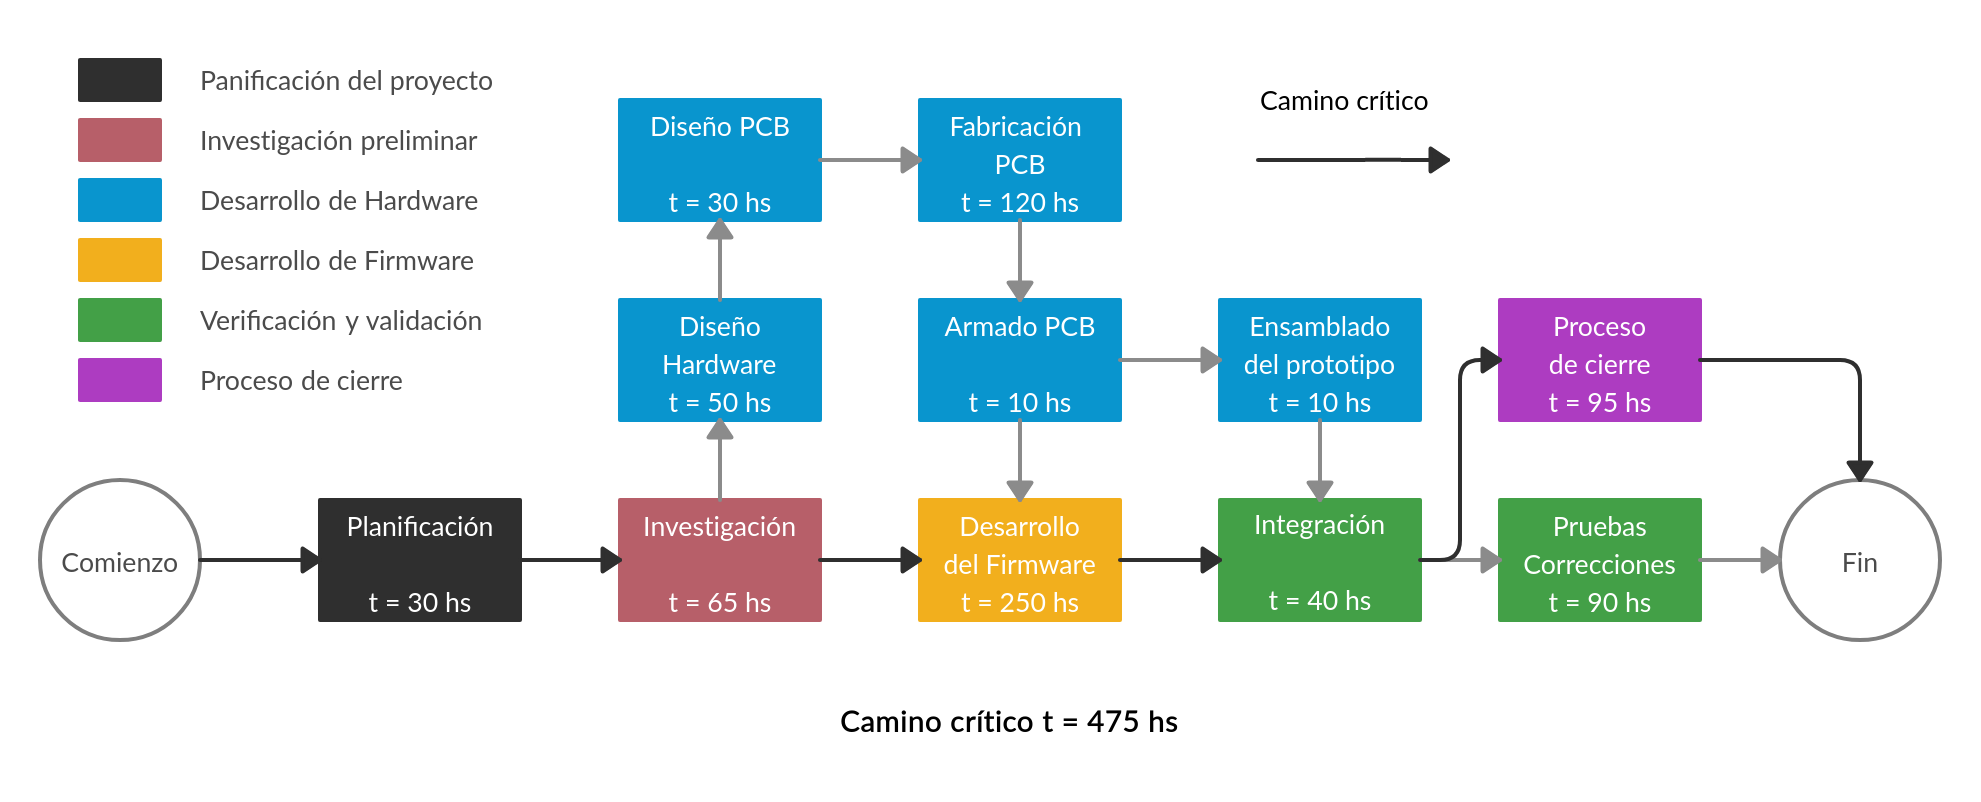
\includegraphics[width=1\textwidth]{./Figuras/AoN_Cargador.png}
\caption{Diagrama en \textit{Activity on Node}}
\label{fig:AoN}
\end{figure}

%Indicar claramente en qué unidades están expresados los tiempos.
%De ser necesario indicar los caminos semicríticos y analizar sus tiempos mediante un cuadro.
%Es recomendable usar colores y un cuadro indicativo describiendo qué representa cada color, como se muestra en el siguiente ejemplo:



\section{8. Diagrama de Gantt}
\label{sec:gantt}

\begin{figure}[H]
\centering 
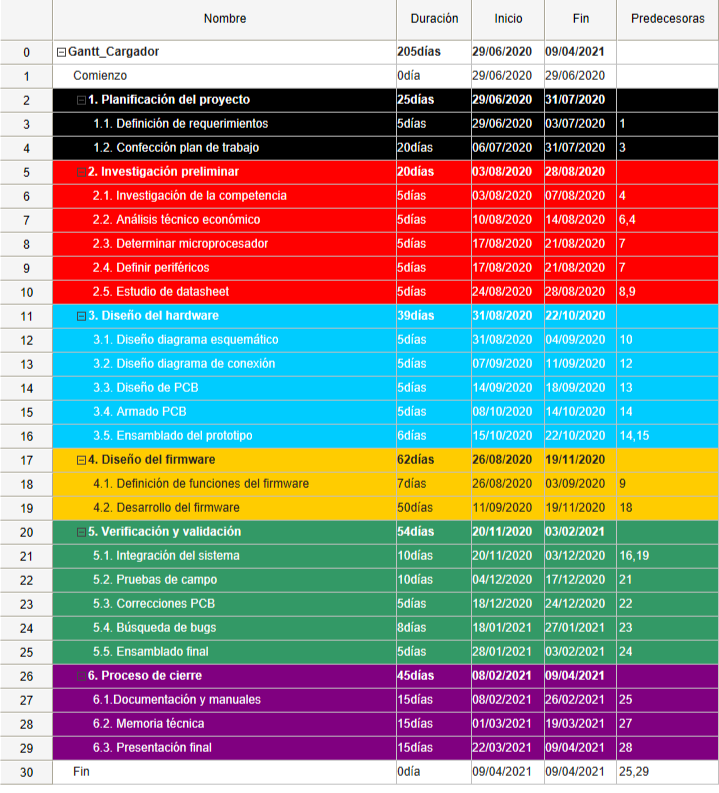
\includegraphics[width=1\textwidth]{./Figuras/Gantt_tabla.png}
\caption{Tabla de tareas}
\label{fig:Tabla Gantt}
\end{figure}

\begin{figure}[H]
\centering 
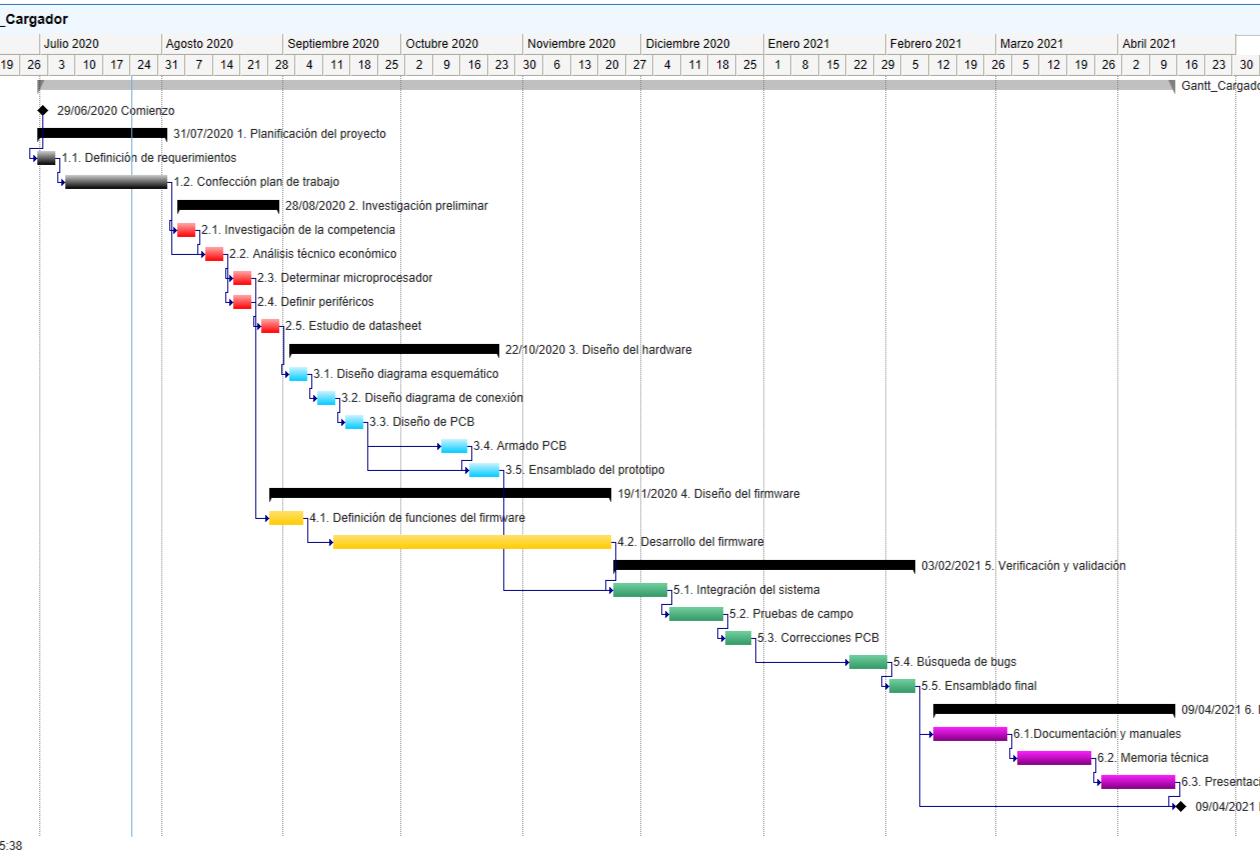
\includegraphics[angle=90, width=1\textwidth]{./Figuras/Gantt_diag.png}
%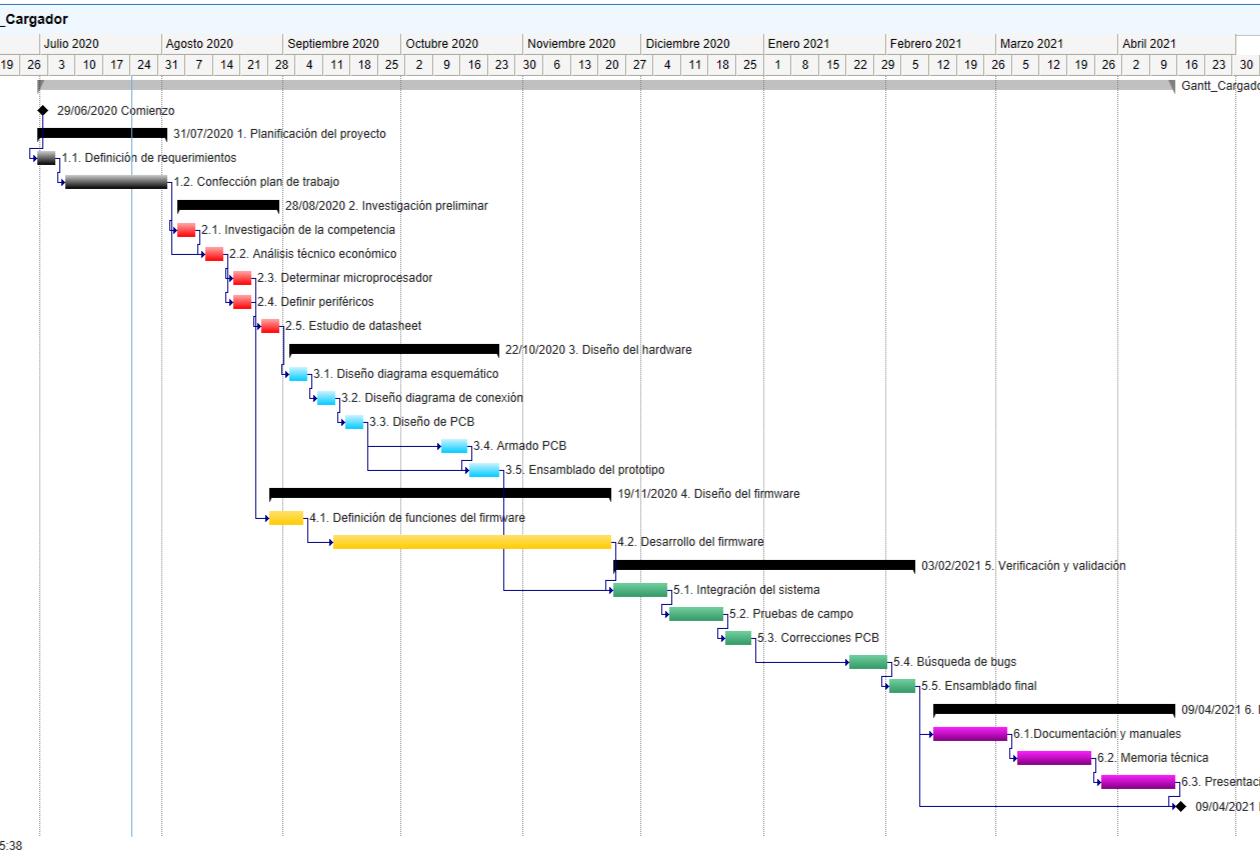
\includegraphics[angle=90]{./Figuras/Gantt_diag.png}
\caption{Diagrama de \textit{Gantt}}
\label{fig:Diagrama Gantt}
\end{figure}

%\begin{consigna}{red}
%Utilizar el software Gantter for Google Drive o alguno similar para dibujar el diagrama de Gantt.

%Existen muchos programas y recursos \textit{online} para hacer diagramas de gantt, entre las cuales destacamos:

%\begin{itemize}
%\item Planner
%\item GanttProject
%\item Trello + \textit{plugins}. En el siguiente link hay un tutorial oficial: \\ \url{https://blog.trello.com/es/diagrama-de-gantt-de-un-proyecto}
%\item Creately, herramienta online colaborativa. \\\url{https://creately.com/diagram/example/ieb3p3ml/LaTeX}
%\item Se puede hacer en latex con el paquete \textit{pgfgantt}\\ \url{http://ctan.dcc.uchile.cl/graphics/pgf/contrib/pgfgantt/pgfgantt.pdf}
%\end{itemize}

%Pegar acá una captura de pantalla del diagrama de Gantt, cuidando que la letra sea suficientemente grande como para ser legible. 
%Si el diagrama queda demasiado ancho, se puede pegar primero la ``tabla'' del Gantt y luego pegar la parte del diagrama de barras del diagrama de Gantt.

%Configurar el software para que en la parte de la tabla muestre los códigos del EDT (WBS).\\
%Configurar el software para que al lado de cada barra muestre el nombre de cada tarea.\\
%Revisar que la fecha de finalización coincida con lo indicado en el Acta Constitutiva.

%En la figura \ref{fig:gantt}, se muestra un ejemplo de diagrama de gantt realizado con el paquete de \textit{pgfgantt}. En la plantilla pueden ver el código que lo genera y usarlo de base para construir el propio.

%\begin{figure}[htbp]
%\begin{center}
%  \gantttitle{2020}{12} \\
%  \gantttitlelist{1,...,12}{1} \\
%  \ganttbar{Task 1}{1}{2} \\
%  \ganttlinkedbar{Task 2}{3}{7} \ganttnewline
%  \ganttmilestone{Milestone o hito}{7} \ganttnewline
%  \ganttbar{Final Task}{8}{12}
%  \ganttlink{elem3}{elem4}
%\end{ganttchart}
%\end{center}
%\caption{Diagrama de gantt de ejemplo}
%\label{fig:gantt}
%\end{figure}

%\end{consigna}

\section{9. Matriz de uso de recursos de materiales}
\label{sec:recursos}


\begin{table}[htpb]
\label{tab:recursos}
\centering
\begin{tabularx}{\linewidth}{@{}|c|l|X|X|X|X|@{}}
\hline

\cellcolor[HTML]{C0C0C0} & \cellcolor[HTML]{C0C0C0} & \multicolumn{4}{c|}{\cellcolor[HTML]{C0C0C0}Recursos requeridos (horas)} \\ \cline{3-6} 

%\cellcolor[HTML]{C0C0C0}WBS & \cellcolor[HTML]{C0C0C0}Tarea &  PC  & Placa PCB & Prototipo & Laboratorio \\ \hline



\multirow{-2}{*}{\cellcolor[HTML]{C0C0C0}\begin{tabular}[c]{@{}c@{}}Código\\ WBS\end{tabular}} & 
\multirow{-2}{*}{\cellcolor[HTML]{C0C0C0}\makebox[4.5cm][c]{Nombre de la tarea}} & 
\multicolumn{1}{|c|}{PC}  &\multicolumn{1}{|c|}{Placa PCB} &\multicolumn{1}{|c|}{Prototipo} &\multicolumn{1}{|c|}{Laboratorio} \\ \hline
  

 \rowcolor[HTML]{000000} 
 \textcolor{white}{1.} &
 \multicolumn{5}{|l|}{\textcolor{white}{Planificación del proyecto}}\\ \cline{1-6}
 
 1.1. &Definición requerimientos &\multicolumn{1}{|c|}{15 hs}  &  &  &  \\ \hline
 1.2. &Plan de trabajo &\multicolumn{1}{|c|}{15 hs} &  &  &  \\ \hline

 \rowcolor[HTML]{FF0000}
 2. & 	
 \multicolumn{5}{|l|}{Investigación preliminar} \\ \cline{1-6}
 
 2.1. &Info de la competencia  &\multicolumn{1}{|c|}{5 hs} &  &  &  \\ \hline
 2.2. &A. técnico-económico  &\multicolumn{1}{|c|}{10 hs} &  &  &  \\ \hline
 2.3. &Determinar microprocesador  &\multicolumn{1}{|c|}{10 hs} &  &  &  \\ \hline
 2.4. &Determinar periféricos  &\multicolumn{1}{|c|}{15 hs} &  &  &  \\ \hline
 2.5. &Estudio datasheet  &\multicolumn{1}{|c|}{25 hs} &  &  &  \\ \hline
 
 \rowcolor[HTML]{00D8FF}
 3. &
 \multicolumn{5}{|l|}{Desarrollo del hardware}	\\ \cline{1-6}
 
 3.1. &Diseño Esquemático &\multicolumn{1}{|c|}{30 hs} &  &  &  \\ \hline
 3.2. &Diseño diagrama conexión &\multicolumn{1}{|c|}{20 hs} &  &  &  \\ \hline
 3.3. &Diseño PCB  &\multicolumn{1}{|c|}{30 hs} &  &  &  \\ \hline
 3.4. &Armado PCB  &  &  &  &\multicolumn{1}{|c|}{10 hs}  \\ \hline
 3.5. &Ensamblado del prototipo  &  &  &  &\multicolumn{1}{|c|}{10 hs} \\ \hline
 
 \rowcolor[HTML]{FFD200}
 4. &
 \multicolumn{5}{|l|}{Desarrollo del firmware}\\ \cline{1-6}
 
 4.1. &Funciones del firmware  &\multicolumn{1}{|c|}{30 hs} &  &  &  \\ \hline
 4.2. &Modularización del código &\multicolumn{1}{|c|}{185 hs} &\multicolumn{1}{|c|}{30 hs}  &  &\multicolumn{1}{|c|}{5 hs}  \\ \hline
 
 \rowcolor[HTML]{00FF00}
 5. &
 \multicolumn{5}{|l|}{Verificación y validación}\\ \cline{1-6}
 
 5.1. &Integración del sistema  &\multicolumn{1}{|c|}{5 hs} &\multicolumn{1}{|c|}{10hs}  &\multicolumn{1}{|c|}{20 hs}  &\multicolumn{1}{|c|}{5 hs} \\ \hline
 5.2. &Prueba de campo  &  &  &  &\multicolumn{1}{|c|}{40 hs}  \\ \hline
 5.3. &Corrección PCB  &\multicolumn{1}{|c|}{5 hs} &\multicolumn{1}{|c|}{5 hs} &  &  \\ \hline
 5.4. &Búsqueda de bugs  &\multicolumn{1}{|c|}{20 hs} &\multicolumn{1}{|c|}{10 hs} &  &  \\ \hline
 5.5. &Ensamble final  &  &  &\multicolumn{1}{|c|}{10 hs} &  \\ \hline
 
 \rowcolor[HTML]{800080}
 \textcolor{white}{6. } &
 \multicolumn{5}{|l|}{\textcolor{white}{Proceso de cierre }}	\\ \cline{1-6} 
 
 6.1. &Documentación y manuales  &\multicolumn{1}{|c|}{20 hs} &  &  &  \\ \hline
 6.2. &Memoria técnica  &\multicolumn{1}{|c|}{60 hs} &  &  &  \\ \hline
 6.3. &Presentación final  &\multicolumn{1}{|c|}{15 hs} &  &  &  \\ \hline    

 \rowcolor[HTML]{C0C0C0}
 \multicolumn{2}{|c|}{\textbf{Totales }} &\multicolumn{1}{|c|}{\textbf{515 hs}}	&\multicolumn{1}{|c|}{\textbf{55 hs}}	&\multicolumn{1}{|c|}{\textbf{30 hs}}	&\multicolumn{1}{|c|}{\textbf{70 hs}}	\\ \cline{1-6}

\end{tabularx}
\end{table}

\begin{itemize}
 \item PC: Computadora con las aplicaciones necesarias para el diseño del hardware y firmware.
 \item Placa PCB: placa de circuito impreso funcional con microprocesador y periféricos.
 \item Prototipo: Placa de control integrada al hardware del cargador
 \item Laboratorio: Espacio físico con instrumental de medición.
\end{itemize}


\section{10. Presupuesto detallado del proyecto}
\label{sec:presupuesto}

%\begin{consigna}{red}
%Si el proyecto es complejo entonces separarlo en partes:
%\begin{itemize}
%\item Un total global, indicando el subtotal acumulado por cada una de las áreas.
%\item El desglose detallado del subtotal de cada una de las áreas.
%\end{itemize}

%IMPORTANTE: No olvidarse de considerar los COSTOS INDIRECTOS.

%\end{consigna}

\begin{table}[H]
\centering
\begin{tabularx}{\linewidth}{@{}|X|c|r|r|@{}}
\hline
\rowcolor[HTML]{C0C0C0} 
\multicolumn{4}{|c|}{\cellcolor[HTML]{C0C0C0}\textbf{COSTOS DIRECTOS}} \\ \hline
\rowcolor[HTML]{C0C0C0} 
Descripción &
  \multicolumn{1}{c|}{\cellcolor[HTML]{C0C0C0}Cantidad} &
  \multicolumn{1}{c|}{\cellcolor[HTML]{C0C0C0}Valor unitario} &
  \multicolumn{1}{c|}{\cellcolor[HTML]{C0C0C0}Valor total} \\ \hline
 
 Fuentes de carga &
  \multicolumn{1}{c|}{3} &
  \multicolumn{1}{r|}{\$ 26.950} &
  \multicolumn{1}{r|}{\$ 80.850} \\ \hline
 
 PCB &
  \multicolumn{1}{c|}{2} &
  \multicolumn{1}{r|}{\$ 4.620} &
  \multicolumn{1}{r|}{\$ 9.240} \\ \hline
 
 Sensor de corriente &
  \multicolumn{1}{c|}{3} &
  \multicolumn{1}{r|}{\$ 924} &
  \multicolumn{1}{r|}{\$ 2.772} \\ \hline
  
 Sensor de tenperatura &
  \multicolumn{1}{c|}{2} &
  \multicolumn{1}{r|}{\$ 153} &
  \multicolumn{1}{r|}{\$ 306} \\ \hline 
  
 Pantalla LCD &
  \multicolumn{1}{c|}{2} &
  \multicolumn{1}{r|}{\$ 1.155} &
  \multicolumn{1}{r|}{\$ 2.310} \\ \hline
  
 Placa de evaluación &
  \multicolumn{1}{c|}{1} &
  \multicolumn{1}{r|}{\$ 2.541} &
  \multicolumn{1}{r|}{\$ 2.541} \\ \hline 
  
 Módulo WIFI &
  \multicolumn{1}{c|}{2} &
  \multicolumn{1}{r|}{\$ 800} &
  \multicolumn{1}{r|}{\$ 800} \\ \hline 
  
 Componentes electrónicos varios (*) &
  \multicolumn{1}{c|}{1} &
  \multicolumn{1}{r|}{\$ 3.000} &
  \multicolumn{1}{r|}{\$ 3.000} \\ \hline
  
 Electricidad y conexionado (*)&
  \multicolumn{1}{c|}{1} &
  \multicolumn{1}{r|}{\$ 2.500} &
  \multicolumn{1}{r|}{\$ 2.500} \\ \hline
 
 Honorario profecional &
  \multicolumn{1}{c|}{670 hs} &
  \multicolumn{1}{r|}{\$ 750} &
  \multicolumn{1}{r|}{\$ 502.500} \\ \hline
  
%\multicolumn{1}{|l|}{} & & & \\ \hline

%\multicolumn{1}{|l|}{} & & & \\ \hline 
      
  \multicolumn{3}{|l|}{SUBTOTAL} &
  \multicolumn{1}{r|}{\$ 605.969} \\ \hline
  
  \rowcolor[HTML]{C0C0C0} 
  \multicolumn{4}{|c|}{\cellcolor[HTML]{C0C0C0}\textbf{COSTOS INDIRECTOS}} \\ \hline
  \rowcolor[HTML]{C0C0C0} 
  Descripción &
  \multicolumn{1}{c|}{\cellcolor[HTML]{C0C0C0}Cantidad} &
  \multicolumn{1}{c|}{\cellcolor[HTML]{C0C0C0}Valor unitario} &
  \multicolumn{1}{c|}{\cellcolor[HTML]{C0C0C0}Valor total} \\ \hline

  \multicolumn{1}{|l|}{Servicios y alquileres} & 10
  & \$ 7.500
  & \$ 75.000
  \\ \hline

  \multicolumn{1}{|l|}{Baterías para pruebas de campo} & 4
  & \$ 19.000
  & \$ 76.000
  \\ \hline
   
  \multicolumn{1}{|l|}{Gastos de aduana e importación} & 1
  & \$ 34.650
  & \$ 34.650 \\ \hline
   
  \multicolumn{1}{|l|}{Certificaciones para la importación} & 1
  & \$ 54.000
  & \$ 54.000 \\ \hline    
   
  \multicolumn{3}{|l|}{SUBTOTAL} &
  \multicolumn{1}{r|}{\$ 239.650} \\ \hline
  \rowcolor[HTML]{C0C0C0}
  \multicolumn{3}{|r|}{\textbf{TOTAL}} & \textbf{\$ 845.619}
  \\ \hline
  
 \end{tabularx}
\end{table}

(*) Valores aproximados

%\pagebreak

\section{11. Matriz de asignación de responsabilidades}
\label{sec:responsabilidades}
%\begin{consigna}{red}
%Establecer la matriz de asignación de responsabilidades y el manejo de la autoridad completando la siguiente tabla:



\begin{table}[H]
 \centering
 \resizebox{\textwidth}{!}{
 \begin{tabular}{|c|l|c|c|c|c|}
  \hline
  \rowcolor[HTML]{C0C0C0} 
  &
  &
  \multicolumn{4}{|c|}{Nombres y roles del proyecto} \\  \cline{3-6}
  
  \rowcolor[HTML]{C0C0C0} 
  &
  &
  Responsable &
  Orientador &
  Equipo &
  Cliente \\ \cline{3-6}
   
\rowcolor[HTML]{C0C0C0} 
\multirow{-3}{*}{\cellcolor[HTML]{C0C0C0}\begin{tabular}[c]{@{}c@{}}Código\\ WBS\end{tabular}} &
  \multirow{-3}{*}{\cellcolor[HTML]{C0C0C0}\makebox[4.5cm][c]{Nombre de la tarea}} &
  \authorname &
  \supname &
  Luca Calcavecchia &
  \clientename \\ \hline

\rowcolor[HTML]{000000} 
 \textcolor{white}{1.} &
 \multicolumn{5}{|l|}{\textcolor{white}{Planificación del proyecto}}\\ \cline{1-6}
 
 1.1. &Definición requerimientos & P  & I & S & P / A \\ \hline
 1.2. &Plan de trabajo & P & C / A & S & I \\ \hline

 \rowcolor[HTML]{FF0000}
 2. & 	
 \multicolumn{5}{|l|}{Investigación preliminar} \\ \cline{1-6}
 
 2.1. &Info de la competencia  & P  & - & S & C \\ \hline
 2.2. &A. técnico-económico  & S & - & - & P  \\ \hline
 2.3. &Determinar microprocesador  & P & A & - & I \\ \hline
 2.4. &Determinar periféricos  & P / A & C & - & - \\ \hline
 2.5. &Estudio datasheet  & P & - & - & - \\ \hline
 
 \rowcolor[HTML]{00D8FF}
 3. &
 \multicolumn{5}{|l|}{Desarrollo del hardware}	\\ \cline{1-6}
 
 3.1. &Diseño Esquemático & P & S & - & - \\ \hline
 3.2. &Diseño diagrama conexión & P & - & C & - \\ \hline
 3.3. &Diseño PCB  & P / A & C & S & I \\ \hline
 3.4. &Armado PCB  & P & I & - & I  \\ \hline
 3.5. &Ensamblado del prototipo & P & I & S & I \\ \hline
 
 \rowcolor[HTML]{FFD200}
 4. &
 \multicolumn{5}{|l|}{Desarrollo del firmware}\\ \cline{1-6}
 
 4.1. &Funciones del firmware  & P & C & - & - \\ \hline
 4.2. &Modularización del código & P & C / A  & - & - \\ \hline
 
 \rowcolor[HTML]{00FF00}
 5. &
 \multicolumn{5}{|l|}{Verificación y validación}\\ \cline{1-6}
 
 5.1. &Integración del sistema  & P & A  & S  & I \\ \hline
 5.2. &Prueba de campo  & P & I & S & A  \\ \hline
 5.3. &Corrección PCB  & P / A & I & - & - \\ \hline
 5.4. &Búsqueda de bugs  & P & C & - & - \\ \hline
 5.5. &Ensamble final  & P & I & P & A \\ \hline
 
 \rowcolor[HTML]{800080}
 \textcolor{white}{6. } &
 \multicolumn{5}{|l|}{\textcolor{white}{Proceso de cierre }}	\\ \cline{1-6} 
 
 6.1. &Documentación y manuales  & P & C & S & A \\ \hline
 6.2. &Memoria técnica  & P & A & - & I \\ \hline
 6.3. &Presentación final  & P & A & - & I \\ \hline    


\end{tabular}%
}
\end{table}

{\footnotesize
Referencias:
\begin{itemize}
	\item P = Responsabilidad Primaria
	\item S = Responsabilidad Secundaria
	\item A = Aprobación
	\item I = Informado
	\item C = Consultado
\end{itemize}
} %footnotesize

\vspace{20px}

%Una de las columnas debe ser para el Director, ya que se supone que participará en el proyecto.
%A su vez se debe cuidar que no queden muchas tareas seguidas sin ``A'' o ``I''.

%Importante: es redundante poner ``I/A'' o ``I/C'', porque para aprobarlo o responder consultas primero la persona debe ser informada.

%\end{consigna}

\section{12. Gestión de riesgos}
\label{sec:riesgos}

A continuación se detallan cinco posibles riesgos inherentes al proyecto. Los mismos son evaluados según su grado de severidad y su probabilidad de ocurrencia tomando valores de 1 a 10. 


\vspace{0.5cm}


\begin{table}[H]
\centering

\begin{tabularx}{\linewidth}{@{}|l|c|X|@{}}
\hline
\rowcolor[HTML]{C0C0C0} 
\multicolumn{3}{c|}{\cellcolor[HTML]{C0C0C0}\textbf{Riesgo 1: Retrasos en las tareas realizadas por el equipo}}  \\ \hline
Severidad  & 9 & No cumplir lo acordado con el cliente. Se disminuye el TIR (tasa interna de retorno). Se pierden posibles ventas. \\ \hline
Ocurrencia & 5 & No se planificó correctamente los tiempos. La curva de aprendizaje se retrasa. Mala coordinación del equipo de trabajo. \\ \hline

\end{tabularx}
\end{table}

\vspace{0.5cm}

\begin{table}[H]
\centering

\begin{tabularx}{\linewidth}{@{}|l|c|X|@{}}
\hline
\rowcolor[HTML]{C0C0C0} 
\multicolumn{3}{c|}{\cellcolor[HTML]{C0C0C0}\textbf{Riesgo 2: Demora en la entrega de insumos}}  \\ \hline
Severidad  & 7 & Desabastecimiento del mercado electrónico local. Demoras aduaneras en la importación.  \\ \hline
Ocurrencia & 8 & Es muy común con los proveedores locales. Modificaciones de las regulaciones aduaneras. \\ \hline

\end{tabularx}
\end{table}

\vspace{0.5cm}

\begin{table}[H]
\centering

\begin{tabularx}{\linewidth}{@{}|l|c|X|@{}}
\hline
\rowcolor[HTML]{C0C0C0} 
\multicolumn{3}{c|}{\cellcolor[HTML]{C0C0C0}\textbf{Riesgo 3: Pérdida de información}}  \\ \hline
Severidad  & 7 & Por desperfectos  de la PC de desarrollo. Robo \\ \hline
Ocurrencia & 3 & Es poco probable si se usa un sistema de control de versiones y/o backup en la nube según sea el caso. \\ \hline

\end{tabularx}
\end{table}

\vspace{0.5cm}

\begin{table}[H]
\centering

\begin{tabularx}{\linewidth}{@{}|l|c|X|@{}}
\hline
\rowcolor[HTML]{C0C0C0} 
\multicolumn{3}{c|}{\cellcolor[HTML]{C0C0C0}\textbf{Riesgo 4: Rotura del prototipo}}  \\ \hline
Severidad  & 9 & Roturas por accidentes en la manipulación. Mal armado. Errores de conexión. Deficiencias en el diseño.  \\ \hline
Ocurrencia & 4 & Si no se usan instalaciones de pruebas adecuadas. Apuros por terminar rápido una tarea. No se dio la suficiente importancia al diseño del hardward.
 \\ \hline

\end{tabularx}
\end{table}

\vspace{0.5cm}

\begin{table}[H]
\centering

\begin{tabularx}{\linewidth}{@{}|l|c|X|@{}}
\hline
\rowcolor[HTML]{C0C0C0} 
\multicolumn{3}{c|}{\cellcolor[HTML]{C0C0C0}\textbf{Riesgo 5: Selección del procesador y/o periféricos}}  \\ \hline
Severidad  & 4 & Las características no alcanzan para cumplir el objetivo, como ser poca capacidad de memoria, pocos GPIO o baja resolución del ADC.  \\ \hline
Ocurrencia & 5 & No poseer suficiente experiencia en este tipo de tecnología. La respuesta de los distintos sensores no es la esperada. 
 \\ \hline

\end{tabularx}
\end{table}

\vspace{0.5cm}

Estos riesgos se ponderan de acuerdo a la siguiente fórmula:

\begin{center}
RPN = S * O
\end{center}


A continuacion se muestra una tabla de gestión de riesgos:      

\begin{table}[htpb]
\centering
\begin{tabularx}{\linewidth}{@{}|X|c|c|c|c|c|c|@{}}
\hline
\rowcolor[HTML]{C0C0C0} 
Riesgo & S & O & RPN & S* & O* & RPN* \\ \hline
 1: Retrasos en las tareas realizadas por el equipo     & 9  & 5  & \textcolor{red}{ 45 }    & 9   & 2   & 18     \\ \hline
 2: Demora en la entrega de insumos     & 7  & 8  &\textcolor{red}{ 56 } & 3   & 8   & 24     \\ \hline
 3: Pérdida de información     & 7  & 3  & 21    &     &     &      \\ \hline
 4: Rotura del prototipo     & 9  & 4  &\textcolor{red}{ 36 }   & 5   & 3 & 15    \\ \hline
 5: Selección del procesador y/o periféricos     & 4  & 5  & 20    &     &     &      \\ \hline

\end{tabularx}%
\end{table}

Criterio adoptado: 
Se tomarán medidas de mitigación en los riesgos cuyos números de RPN sean mayores a 30

Nota: los valores marcados con (*) en la tabla corresponden luego de haber aplicado la mitigación.

Como se observa en la tabla vemos que tres de los cinco riesgos no cumplen el criterio. 
A continuación analizaremos como mitigar los riesgos con RPN mayor a 30.

\begin{table}[H]
\centering

\begin{tabularx}{\linewidth}{@{}|l|c|X|@{}}
\hline
\rowcolor[HTML]{C0C0C0} 
\multicolumn{3}{c|}{\cellcolor[HTML]{C0C0C0}\textbf{Riesgo 1: Retrasos en las tareas realizadas por el equipo}}  \\ \hline
Severidad  & 9 & La severidad sigue siendo la misma que antes de la mitigación. \\ \hline
Ocurrencia & 2 & Se puede reordenar la distribución de horas de trabajo. Se pide asesoramiento al director del proyecto para los temas que generan mayores dudas. Para mejorar la relacion con el equipo se pueden implementar conceptos aprendidos en metodologías ágiles y scrum. \\ \hline

\end{tabularx}
\end{table}

\vspace{0.5cm}

\begin{table}[H]
\centering

\begin{tabularx}{\linewidth}{@{}|l|c|X|@{}}
\hline
\rowcolor[HTML]{C0C0C0} 
\multicolumn{3}{c|}{\cellcolor[HTML]{C0C0C0}\textbf{Riesgo 2: Demora en la entrega de insumos}}  \\ \hline
Severidad  & 3 & Se puede bajar la severidad, generando las compras con mayor antelación. Gestionar las importaciones con los proveedores locales. Dentro de lo posible adaptarse a los insumos que se consiguen en el mercado local \\ \hline
Ocurrencia & 8 & La ocurrencia no cambia porque seguimos dependiendo de terceros. \\ \hline

\end{tabularx}
\end{table}

\vspace{0.5cm}

\begin{table}[H]
\centering

\begin{tabularx}{\linewidth}{@{}|l|c|X|@{}}
\hline
\rowcolor[HTML]{C0C0C0} 
\multicolumn{3}{c|}{\cellcolor[HTML]{C0C0C0}\textbf{Riesgo 4: Rotura del prototipo}}  \\ \hline
Severidad  & 5 & Se baja la severidad armando al menos dos prototipos (redundancia del 100\%).  \\ \hline
Ocurrencia & 3 & Se puede bajar la ocurrencia maximizando los cuidados en la manipulación y los ensayos. Minimizar la precariedad.
 \\ \hline

\end{tabularx}
\end{table}

\vspace{0.5cm}

\section{13. Gestión de la calidad}
\label{sec:calidad}

\begin{enumerate}
	\item \textbf{Requerimientos generales del proyecto}
	\begin{enumerate}[label*=\arabic*.]
		\item Fecha de entrega del proyecto terminado: 5 de Julio de 2021.
		
		\textbf{-Verificación:} Se verifica acorde al diagrama de Gantt.
		
		\textbf{-Validación:} Es tarea del cliente y del director del proyecto hacer el seguimiento.
		
		\item El responsable asegura al cliente el know-how del proyecto.
		
		\textbf{-Verificación:} Se irán entregando los avances del proyecto al cliente
		
		\textbf{-Validación:} El cliente dará conformidad a la documentación entregada
		
		\item Podrá alimentarse con línea de red monofásica o trifásica.
		
		\textbf{-Verificación:} Se verificará que el prototipo tenga conexión para los tipos de alimentación.
		
		\textbf{-Validación:} Se hará en las pruebas de campo. El prototipo debe responder indistintamente con ambos tipos de alimentación.
		
		\item Deberá contemplar protecciones de alimentación a través de llaves térmicas.
		
		\textbf{-Verificación:} Se realiza cálculo de consumo a plena carga.
		
		\textbf{-Validación:} Se realiza prueba de corto circuito con Variac y amperímetro.
		
	\end{enumerate}

	\item \textbf{Requerimientos funcionales}
	\begin{enumerate}[label*=\arabic*.]
		\item \textbf{Requerimientos de Hardware}
			\begin{enumerate}[label*=\arabic*.]
				\item El dispositivo debe contemplar un diseño modular.
				
				\textbf{-Verificación:} Se verifica que el diseño se adapte para conectar múltiples fuente de carga.
		
				\textbf{-Validación:}  Se hace funcionar el cargador con una, dos y hasta tres fuentes de carga.
		
				\item El diseño modular debe permitir su re configuración.
				
				
				\textbf{-Verificación:} Ídem 2.1.1.
		
				\textbf{-Validación:} Las pruebas de campo se harán conectando una, dos o tres fuentes de carga y comprobando el funcionamiento en los tres casos.
		
				\item Debe tener un teclado accesible para su configuración y manejo.
				
				\textbf{-Verificación:} Se puede verificar simulando el código o directamente en la placa de control presionando todas las teclas y verificando si responden.
		
				\textbf{-Validación:} Se comprueba en el prototipo que las teclas ejecutan las acciones  para las que fueron encomendadas.
				
				\item Debe poseer un display que permita visualizar la configuración y parámetros mensurables.
				
				\textbf{-Verificación:} Se verifica el encuadre, brillo y contraste.
		
				\textbf{-Validación:} Se comprueba el funcionamiento sincronizado con el teclado y que los valores mensurables sean los correctos (alineación, decimales, unidades, decenas y centenas).
				
				\item Debe poseer indicadores luminosos bien visibles.
				
				\textbf{-Verificación:} Se verifica que enciendan y apaguen.
		
				\textbf{-Validación:} Se comprueba que se correspondan a las funciones asociadas.
									
				\item Cada fuente debe tener su propio sensor de corriente.
				
				\textbf{-Verificación:} Se verifica que respondan a los estímulos y su correcta polaridad.
		
				\textbf{-Validación:} Se comprueba su precision y exactitud según hoja de datos. 
				
				\item El sensor de tensión es común a todas las fuentes.
				
				\textbf{-Verificación:} Se verifica que responda a los estímulos y su correcta polaridad .
		
				\textbf{-Validación:} Se comprueba su precision y exactitud.
				
				\item Se agrega un botón de parada de emergencia.
				
				\textbf{-Verificación:} Se simula su accionamiento y que responda deteniendo el proceso de carga.
		
				\textbf{-Validación:} Se mide que el tiempo de respuesta sea el correcto.
							
			\end{enumerate}
		\item \textbf{Requerimientos de Firmware}
			\begin{enumerate}[label*=\arabic*.]
				\item Debe permitir configurar la tensión y corriente máxima de carga.
				
				\textbf{-Verificación:} Se simula una configuración de batería y se  verifica que tengan un límite máximo.
		
				\textbf{-Validación:} Se comprueba que los límites máximos sean los que correspondan a cada etapa de carga.
				
				\item Debe permitir configurar los tiempos máximos para cada etapa de carga.
							
				\textbf{-Verificación:} Se verifica que los procesos de carga finalicen por tiempo, haciendo simulaciones con tiempos de carga mas cortos a los reales.
		
				\textbf{-Validación:} Se mide los tiempos de los distintos pasos de carga y se comprueba que sean los correctos.
				
				\item Debe guardar al menos dos configuraciones.
				
				
				\textbf{-Verificación:} Se realiza pudiendo cargar los parámetros de dos tipos de baterías distintas.
		
				\textbf{-Validación:} Se controla que cada configuración de batería modifique los parámetros de carga máximos. 
				
				\item Tendrá que medir tensión, corriente y temperatura.
				
				
				\textbf{-Verificación:} Se simulan los datos de los sensores y se visualizan en la pantalla.
		
				\textbf{-Validación:} Se comprueba con un multímetro auxiliar los valores medidos.
				
				\item Tendrá que garantizar cuatro etapas de carga:
					\begin{enumerate}[label*=\arabic*.]
						\item Carga a Fondo.				
						
						\textbf{-Verificación:} Se simula la conexión de una batería y que el detector de comienzo a la carga a fondo . 
		
						\textbf{-Validación:} Se comprueba que la carga se haga a corriente constante y sea la corriente máxima.
				
						\item Carga por Absorción.	
						
						\textbf{-Verificación:} Se realizan simulaciones con tiempos cortos de ejecución verificando el paso de carga a fondo a carga por absorción. 
		
						\textbf{-Validación:} Se comprueba la transición y que la carga se haga a tensión máxima constante.
				
						\item Carga a Flote.
						
						\textbf{-Verificación:} Se realizan simulaciones con tiempos cortos de ejecución verificando el paso de carga por absorción a flote. 
		
						\textbf{-Validación:} Se comprueba la transición y que la tensión no supere el 10\% de la tensión nominal ni el 10\% de la corriente máxima.
						
						\item Ecualización.
						
						\textbf{-Verificación:} Se realizan simulaciones con tiempos cortos de ejecución, verificando el cambio del paso de carga por absorción a ecualización.  
		
						\textbf{-Validación:} Se comprueba la transición y que la tensión no supere el 10\% de la tensión máxima y que la corriente se se limite al 10\% de la corriente máxima.
				
					\end{enumerate}
				\item Tendrá un algoritmo que atienda al botón de parada de emergencia.
				
				\textbf{-Verificación:} Se simula el accionamiento del botón y como responde el programa.
		
				\textbf{-Validación:} Con el prototipo funcionando, se presiona el botón de parada de emergencia, y se comprueba la detención automática la carga y el tiempo que demora. 
				
				\item El control de carga se realizará por un algoritmo PID.
				
				\textbf{-Verificación:} Se determinan las constantes Kp, Ki y Kd y se verifica su comportamiento.
		
				\textbf{-Validación:} Una vez sintonizadas las constantes del PID se comprueba la estabilidad del sistema.
				
				\item Se registrará la fecha y hora de inicio y finalización de cada carga a través de un RTC.
				
				\textbf{-Verificación:} Se realizan simulaciones con tiempos cortos de ejecución de una carga y se verifica que se registren la fecha y hora. 
		
				\textbf{-Validación:} Se comprueba luego de una carga completa que al finalizar se registren la fecha y hora.
				
				\item Debe guardar las últimas mil cargas realizadas.
				
				\textbf{-Verificación:} Se simula la carga de 1000 registros en la EEPROM.
		
				\textbf{-Validación:} Se comprueba la integridad de los 1000 registros grabados.
				
				\item Con los datos recavados se podrá determinar anomalías y generar alarmas.
				
				\textbf{-Verificación:} Se simula un caso particular guardando datos en EEPROM que fuercen el disparo de alarmas.
		
				\textbf{-Validación:} Resulta complicado hacer la validación, por los tiempos que llevaría la comprobación, por lo que que se aceptará si cumple la verificación.
				 
				\item El registro de datos almacenados debe estar disponible para ser consultado remotamente.
				
				\textbf{-Verificación:} Se simula por UART la consulta del registro de datos.
		
				\textbf{-Validación:} Se comprueba enviando el comando de lectura y que el mismo sea recibido por el módulo WIFI. A su vez el módulo WIFI enviará los datos guardados en EEPROM.					
				
			\end{enumerate}					
	\end{enumerate}
	\item \textbf{Requerimientos no funcionales}
	\begin{enumerate}[label*=\arabic*.]
		\item Se deberá generar documentación:
			\begin{enumerate}[label*=\arabic*.]
				\item Esquemáticos eléctricos.
				
				\textbf{-Verificación:} Se verifica que lo documentado se corresponda con el prototipo final.
		
				\textbf{-Validación:} Será validado por el responsable del proyecto.
				
				\item Manual de instalación.
				
				\textbf{-Verificación:} Ídem 3.1.1.
		
				\textbf{-Validación:} Ídem 3.1.1.
				
				\item Manual de uso.
				
				\textbf{-Verificación:} Se verifica que lo documentado se cumpla en la práctica
		
				\textbf{-Validación:} Será validado por el cliente.
				
			\end{enumerate}
		\item Se contará con la correspondiente certificación eléctrica otorgada por un laboratorio habilitado para la importación de las fuentes de carga.
		
		\textbf{-Verificación:} No aplica
		
		\textbf{-Validación:} No aplica
				
		\item El grado de protección del sistema debe ser como mínimo IP50.
		
		\textbf{-Verificación:} Se verifica de acuerdo a lo establecido en la norma 
		
		\textbf{-Validación:} Será validado por el cliente.
				
		\item Se debe garantizar un servicio de post venta por al menos 5 años.
		
		\textbf{-Verificación:} No aplica.
		
		\textbf{-Validación:} No aplica
				
	\end{enumerate}
\end{enumerate}


\section{14. Comunicación del proyecto}
\label{sec:comunicaciones}

El plan de comunicación del proyecto es el siguiente:

% Please add the following required packages to your document preamble:
% \usepackage{graphicx}
% \usepackage[table,xcdraw]{xcolor}
% If you use beamer only pass "xcolor=table" option, i.e. \documentclass[xcolor=table]{beamer}
\begin{table}[htpb]
\centering
\resizebox{\linewidth}{!}{%
\begin{tabular}{|c|c|c|c|c|c|}
\hline
\rowcolor[HTML]{C0C0C0} 
\multicolumn{6}{|c|}{\cellcolor[HTML]{C0C0C0}PLAN DE COMUNICACIÓN DEL PROYECTO}           \\ \hline
\rowcolor[HTML]{C0C0C0} 
¿Qué comunicar? & Audiencia & Propósito & Frecuencia & Comunicación & Responsable \\ \hline

Plan de trabajo & 
\multicolumn{1}{c|}{\begin{tabular}[c]{@{}c@{}}Cliente\\ Director\\ Clase GdP\end{tabular}} & 
\multicolumn{1}{c|}{\begin{tabular}[c]{@{}c@{}}Dar a conocer el proyecto\\ y como se realizará\end{tabular}} &  
Una vez  & 
\multicolumn{1}{c|}{\begin{tabular}[c]{@{}c@{}}Por escrito y/o \\ videoconferencia\end{tabular}} & 
\authorname  \\ \hline

Informe de avance & 
\multicolumn{1}{c|}{\begin{tabular}[c]{@{}c@{}}Cliente\\ Director \end{tabular}} & 
\multicolumn{1}{c|}{\begin{tabular}[c]{@{}c@{}}Informar si las tareas\\ se cumplen en los\\plazos establecidos \end{tabular}} &  
\multicolumn{1}{c|}{\begin{tabular}[c]{@{}c@{}}quincenal-\\ mente\end{tabular}}  & 
\multicolumn{1}{c|}{\begin{tabular}[c]{@{}c@{}}e-mail y/o \\ videoconferencia \end{tabular}} & 
\authorname  \\ \hline
 

Desviaciones & 
\multicolumn{1}{c|}{\begin{tabular}[c]{@{}c@{}} Director \end{tabular}} & 
\multicolumn{1}{c|}{\begin{tabular}[c]{@{}c@{}}Buscar posibles soluciones\\ y re programar tareas\\si fuera necesario \end{tabular}} &  
\multicolumn{1}{c|}{\begin{tabular}[c]{@{}c@{}}Cuando\\ ocurra\end{tabular}}  & 
\multicolumn{1}{c|}{\begin{tabular}[c]{@{}c@{}}e-mail y/o \\ videoconferencia \end{tabular}} & 
\authorname  \\ \hline 
 
\multicolumn{1}{|c|}{\begin{tabular}[c]{@{}c@{}}Presentación del\\ proyecto final\end{tabular}} & 
\multicolumn{1}{c|}{\begin{tabular}[c]{@{}c@{}} Cliente\\Director\\Jurado\end{tabular}} & 
\multicolumn{1}{c|}{\begin{tabular}[c]{@{}c@{}}Exponer el producto final,\\ detallando su diseño \\y construcción \end{tabular}} &  
\multicolumn{1}{c|}{\begin{tabular}[c]{@{}c@{}}Una vez\end{tabular}}  & 
\multicolumn{1}{c|}{\begin{tabular}[c]{@{}c@{}}videoconferencia \end{tabular}} & 
\authorname  \\ \hline 


\end{tabular}%
}
\end{table}

\section{15. Gestión de Compras}
\label{sec:compras}

El presente proyecto no presenta gran complejidad en la adquisición de sus insumos. Los componentes electrónico se consiguen en parte en el mercado local (Elemon, Cika o Semak) y parte en el extranjero (DigiKey, Mean Well). Además el cliente asegura poseer en stock todos los elementos necesarios para la construcción del prototipo.
El único elemento pendiente de compra, a la hora de la creación de este plan de trabajo, es el PCB, que queda supeditado al diseño del mismo.


\section{16. Seguimiento y control}
\label{sec:seguimiento}


\begin{table}[H]
\resizebox{\textwidth}{!}{%
\begin{tabular}{|c|l|c|c|c|c|c|}
\hline
\rowcolor[HTML]{C0C0C0} 
\multicolumn{7}{|c|}{\cellcolor[HTML]{C0C0C0}\textbf{SEGUIMIENTO DEL AVANCE}}                                                                                                                                                                                                                                                                                                                                             \\ \hline
\rowcolor[HTML]{C0C0C0} 
WBS  & Nombre de la tarea    & \begin{tabular}[c]{@{}c@{}}Indicador\\ de avance\end{tabular}   & \begin{tabular}[c]{@{}c@{}}Frecuencia\\ de reporte\end{tabular} & \begin{tabular}[c]{@{}c@{}}Responsable del\\ seguimiento\end{tabular} & \begin{tabular}[c]{@{}c@{}}Persona a ser\\ informada\end{tabular} & Comunicación                                                \\ \hline

1.1. &
\begin{tabular}[l]{@{}l@{}}Definición de los\\  requerimientos\end{tabular} &
\begin{tabular}[c]{@{}c@{}}\% de \\ definiciones\end{tabular} & 
Al finalizar                                                    &                                                                      
\authorname														&                                                                  
\clientename 													& 
\begin{tabular}[c]{@{}c@{}}Reunion \\ personal\end{tabular} \\ \hline

1.2. &
\begin{tabular}[l]{@{}l@{}}Confección del plan\\ de trabajo\end{tabular}           &
\begin{tabular}[c]{@{}c@{}}\% de Ítems\end{tabular}           & 
Al finalizar                                                    &                                                                      
\authorname														&                                                                  
\clientename														& 
e-mail                                                      \\ \hline

2.1. &
\begin{tabular}[l]{@{}l@{}}Información sobre\\ la competencia\end{tabular} &
\begin{tabular}[c]{@{}c@{}}\% del informe\end{tabular}           & 
Al finalizar                                                    &                                                                      
\clientename														&                                                                  
\authorname														& 
\begin{tabular}[c]{@{}c@{}}Reunion \\ personal\end{tabular} \\ \hline

2.2. &
\begin{tabular}[l]{@{}l@{}}Análisis Técnico-\\ Económico\end{tabular}           &
\begin{tabular}[c]{@{}c@{}}\% del informe\end{tabular}           & 
Al finalizar                                                    &                                                                      
\authorname														&                                                                  
\clientename														& 
\begin{tabular}[c]{@{}c@{}}Reunion \\ personal\end{tabular} \\ \hline

2.3. &
\begin{tabular}[l]{@{}l@{}}Análisis sobre\\ el microprocesador\end{tabular}   &
\begin{tabular}[c]{@{}c@{}}\% del análisis\end{tabular}           & 
Semanal                                                    &                                                                      
\authorname														&                                                                  
\supname														& 
e-mail 													\\ \hline

2.4. &
\begin{tabular}[l]{@{}l@{}}Investigación sobre\\ los periféricos\end{tabular}   &
\begin{tabular}[c]{@{}c@{}}\% de la \\investigación\end{tabular}           & 
quincenal                                                    &                                                                      
\authorname														&                                                                  
\supname														& 
e-mail 													\\ \hline


2.5. &
\begin{tabular}[l]{@{}l@{}}Estudio de los data\\sheet de periféricos\end{tabular}   &
\begin{tabular}[c]{@{}c@{}}\% del estudio\end{tabular}           & 
quincenal                                                    &                                                                      
\authorname														&                                                                  
\supname														& 
e-mail 													\\ \hline

3.1. &
\begin{tabular}[l]{@{}l@{}}Diseño del diagrama\\ esquemático\end{tabular}   &
\begin{tabular}[c]{@{}c@{}}\% del diseño\end{tabular}           & 
quincenal                                                   &                                                                      
\authorname														&                                                                  
\supname														& 
e-mail 													\\ \hline

3.2. &
\begin{tabular}[l]{@{}l@{}}Diseño del diagrama\\ de conexión\end{tabular}   &
\begin{tabular}[c]{@{}c@{}}\% del diseño\end{tabular}           & 
quincenal                                                   &                                                                      
\authorname														&                                                                  
\supname														& 
e-mail 													\\ \hline 

3.3. &
\begin{tabular}[l]{@{}l@{}}Diseño de \\los PCB's\end{tabular}   &
\begin{tabular}[c]{@{}c@{}}\% del diseño\end{tabular}           & 
quincenal                                                   &                                                                      
\authorname														&                                                                  
\supname														& 
e-mail 													\\ \hline

3.4. &
\begin{tabular}[l]{@{}l@{}}Armado de \\los PCB's\end{tabular}   &
\begin{tabular}[c]{@{}c@{}}\% de armado\end{tabular}           & 
quincenal                                                   &                                                                      
\authorname														&                                                                  
\supname														& 
e-mail 													\\ \hline

3.5. &
\begin{tabular}[l]{@{}l@{}}Ensamblado del\\prototipo inicial\end{tabular}   &
\begin{tabular}[c]{@{}c@{}}\% de ensamblaje\end{tabular}           & 
quincenal                                                   &                                                                      
\authorname														&                                                                  
\supname														& 
e-mail 													\\ \hline

4.1. &
\begin{tabular}[l]{@{}l@{}}Definición de \\funciones\end{tabular}   &
\begin{tabular}[c]{@{}c@{}}Cantidad de \\funciones\end{tabular}           & 
quincenal                                                   &                                                                      
\authorname														&                                                                  
\supname														& 
e-mail 													\\ \hline

4.2. &
\begin{tabular}[l]{@{}l@{}}Modularización \\del código\end{tabular}   &
\begin{tabular}[c]{@{}c@{}}\% de módulos\\terminados\end{tabular}           & 
quincenal                                                   &                                                                      
\authorname														&                                                                  
\supname														& 
e-mail 													\\ \hline

5.1. &
\begin{tabular}[l]{@{}l@{}}Integración del \\sistema\end{tabular}   &
\begin{tabular}[c]{@{}c@{}}\% de \\integración\end{tabular}           & 
quincenal                                                   &                                                                      
\authorname														&                                                                  
\supname														& 
e-mail 													\\ \hline

5.2. &
\begin{tabular}[l]{@{}l@{}}Pruebas de \\campo\end{tabular}   &
\begin{tabular}[c]{@{}c@{}}Cantidad de \\pruebas\end{tabular}           & 
quincenal                                                   &                                                                      
\authorname														&                                                                  
\begin{tabular}[c]{@{}c@{}}\supname  \\ \clientename\end{tabular}		& 
e-mail 													\\ \hline

5.3. &
\begin{tabular}[l]{@{}l@{}}Corrección de \\los PCB's \end{tabular}   &
\begin{tabular}[c]{@{}c@{}}\% de \\realización\end{tabular}           & 
quincenal                                                   &                                                                      
\authorname														&                                                                  
\supname														& 
e-mail 													\\ \hline

5.4. &
\begin{tabular}[l]{@{}l@{}}Búsqueda de bugs \end{tabular}   &
\begin{tabular}[c]{@{}c@{}}\% de \\realización\end{tabular}           & 
quincenal                                                   &                                                                      
\authorname														&                                                                  
\supname														& 
e-mail 													\\ \hline

5.5. &
\begin{tabular}[l]{@{}l@{}}Ensamblado final \\del prototipo \end{tabular}   &
\begin{tabular}[c]{@{}c@{}}\% de \\ensamblaje\end{tabular}           & 
quincenal                                                   &                                                                      
\authorname														&                                                                  
\supname														& 
e-mail 													\\ \hline

5.3. &
\begin{tabular}[l]{@{}l@{}}Corrección de \\los PCB's \end{tabular}   &
\begin{tabular}[c]{@{}c@{}}\% de \\realizaci\end{tabular}           & 
quincenal                                                   &                                                                      
\authorname														&                                                                  
\supname														& 
e-mail 													\\ \hline

6. &
\begin{tabular}[l]{@{}l@{}}Proceso de \\cierre \end{tabular}   &
\begin{tabular}[c]{@{}c@{}}\% de \\elaboración\end{tabular}           & 
quincenal                                                   &                                                                      
\authorname														&                                                                  
\begin{tabular}[c]{@{}c@{}}\supname  \\ \clientename\\ Jurado\end{tabular}     & 
e-mail 													\\ \hline

\end{tabular}%
}
\end{table}

\section{17. Procesos de cierre}    
\label{sec:cierre}


Se establecerá una reunión con los distintos actores involucrados e interesados en el proyecto donde se contemple las siguientes actividades:

\begin{itemize}
\item El responsable del proyecto, \authorname, analizará junto al director, \supname, el cumplimiento del WBS, los cambios realizados y los tiempos en el que se llevaron a cabo. Se revisarán las técnicas de diseño aplicadas en el proyecto, y se comentarán cuales tuvieron éxito y cuáles no. A su vez se repasarán los problemas enfrentados y como se solucionaron.

\item El responsable del proyecto, \authorname, comunicará al cliente, \clientename, la finalización del proyecto y hará entrega de toda la documentación correspondiente del producto para su producción. También entregará un informe técnico-económico del producto.

\item El responsable del proyecto, \authorname, elaborará un documento con la memoria y una presentación del producto para su defensa pública ante un jurado evaluador. En ella también se agradecerá al director por haber dirigido y controlado todo el trabajo, al cliente por la confianza dispensada y por el aporte financiero y en especial al equipo y colaboradores por su compromiso de trabajo para con el proyecto. 

\end{itemize}



\end{document}
